\documentclass[12pt,a4paper,UKenglish]{article}
\usepackage[utf8]{inputenc}
\usepackage[T1]{fontenc, url}
\usepackage{float}
\usepackage{graphicx}
%\usepackage{siunitx}
\usepackage{babel,csquotes,newcent,textcomp}
\usepackage[backend=biber, sortcites, sorting=none ]{biblatex}
%\usepackage{subfig}
\usepackage{hyperref}
\hypersetup{colorlinks=true, linktoc=none, linkcolor=blue,}


\title{Electrical noise – counter measures and calculation\\
Mandatory task 1}
\author{Rikesh Chauhan\\ 
\texttt{rikesh.chauhan@fys.uio.no}}
\date{}

\begin{document}
\maketitle

%% Task 1
\section{LM741}
%% Task 1a
\subsection{Transient Analysis}
Resistors $R11$ and $R12$ makes a negative feedback network. Inut is applied in the positive terminal, so it is a non-inverting amplifier. 

Since the gain of a non-inverting amplifier is given as $A_v = 1 + R11/R12$, and  $R11$ and $R12$ have values 10K and 1K, the gaon is 11 in theory.

Relation between DC input, AC input, gain and output range...

\begin{figure} [h]
  \centering 
  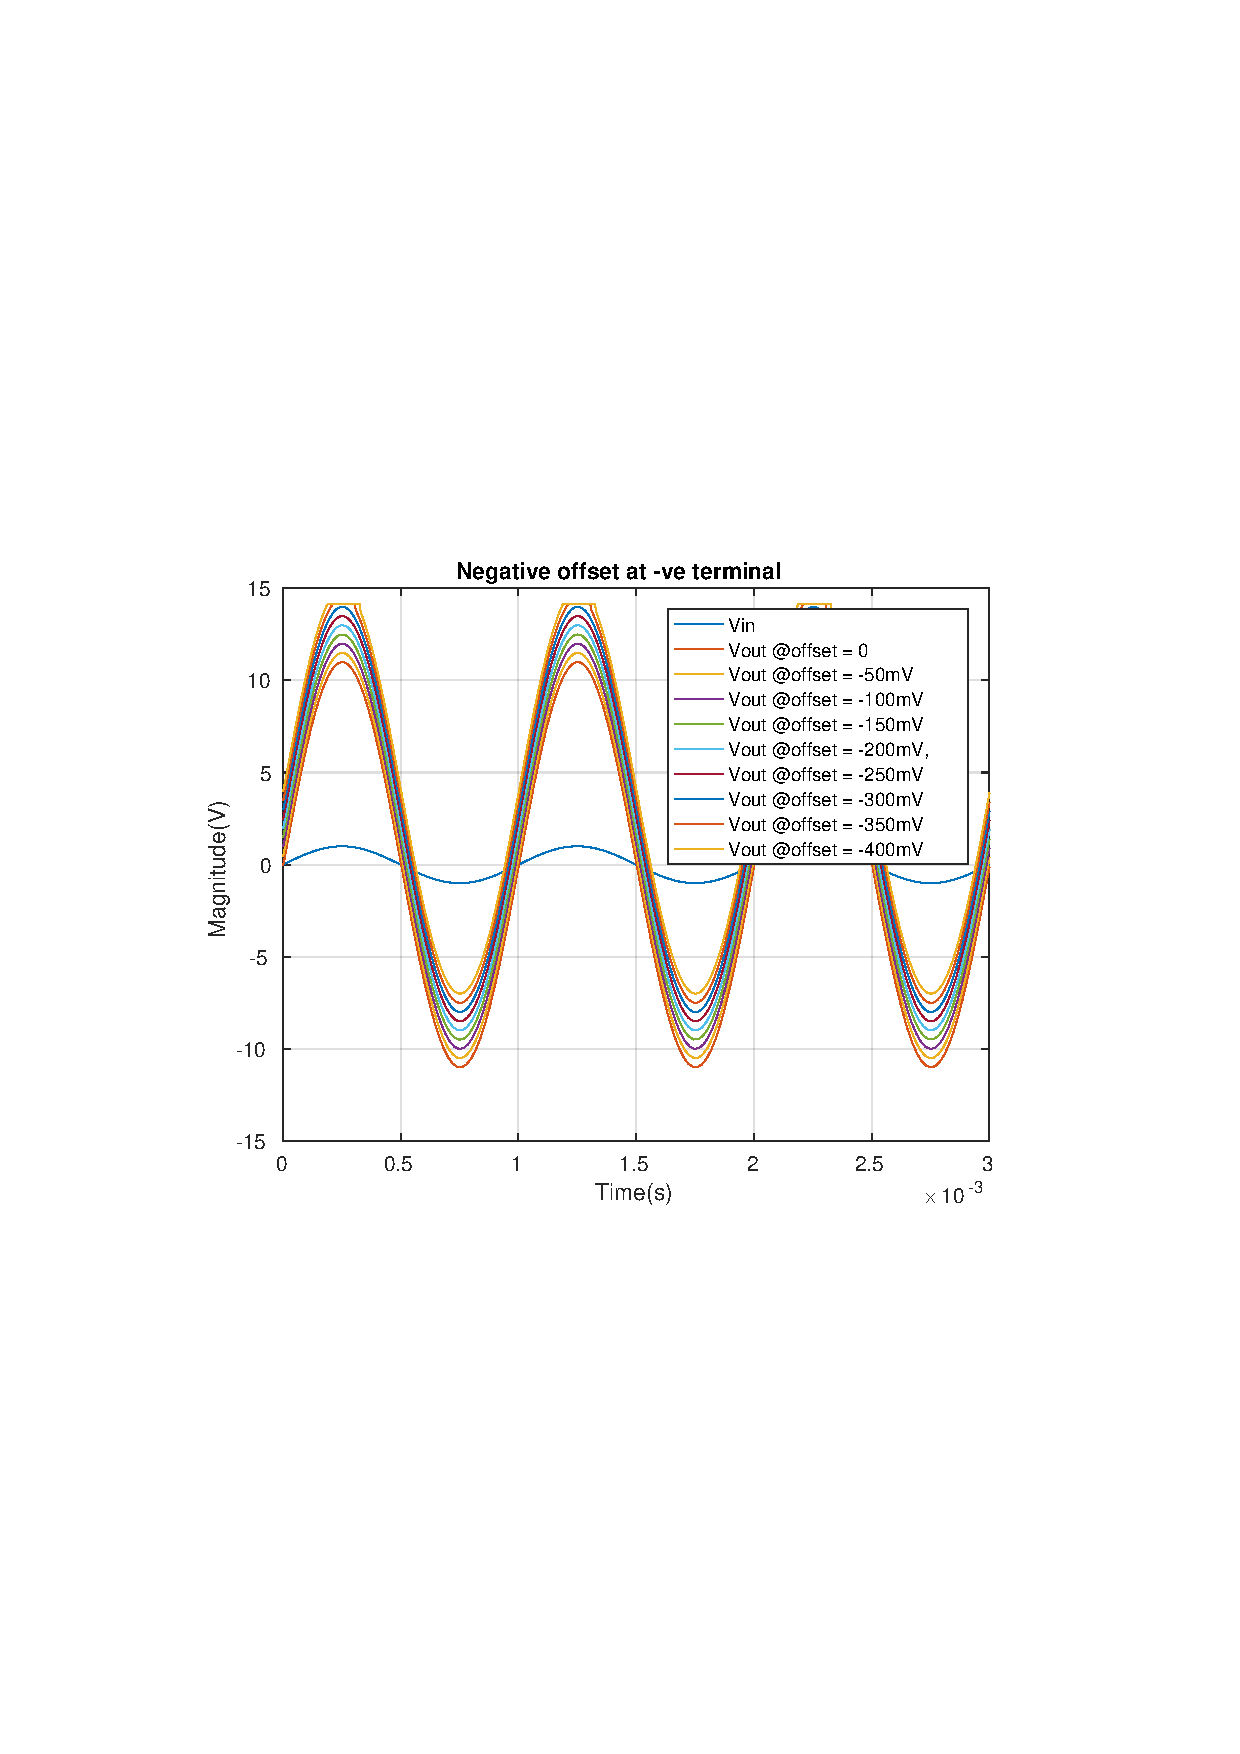
\includegraphics[width=0.9\textwidth]{img/1a_offset_neg.pdf} 
  \caption{Vout with -ve offset at -ve terminal}
  \label{neg_offset} 
\end{figure}

\begin{figure} [h]
  \centering 
  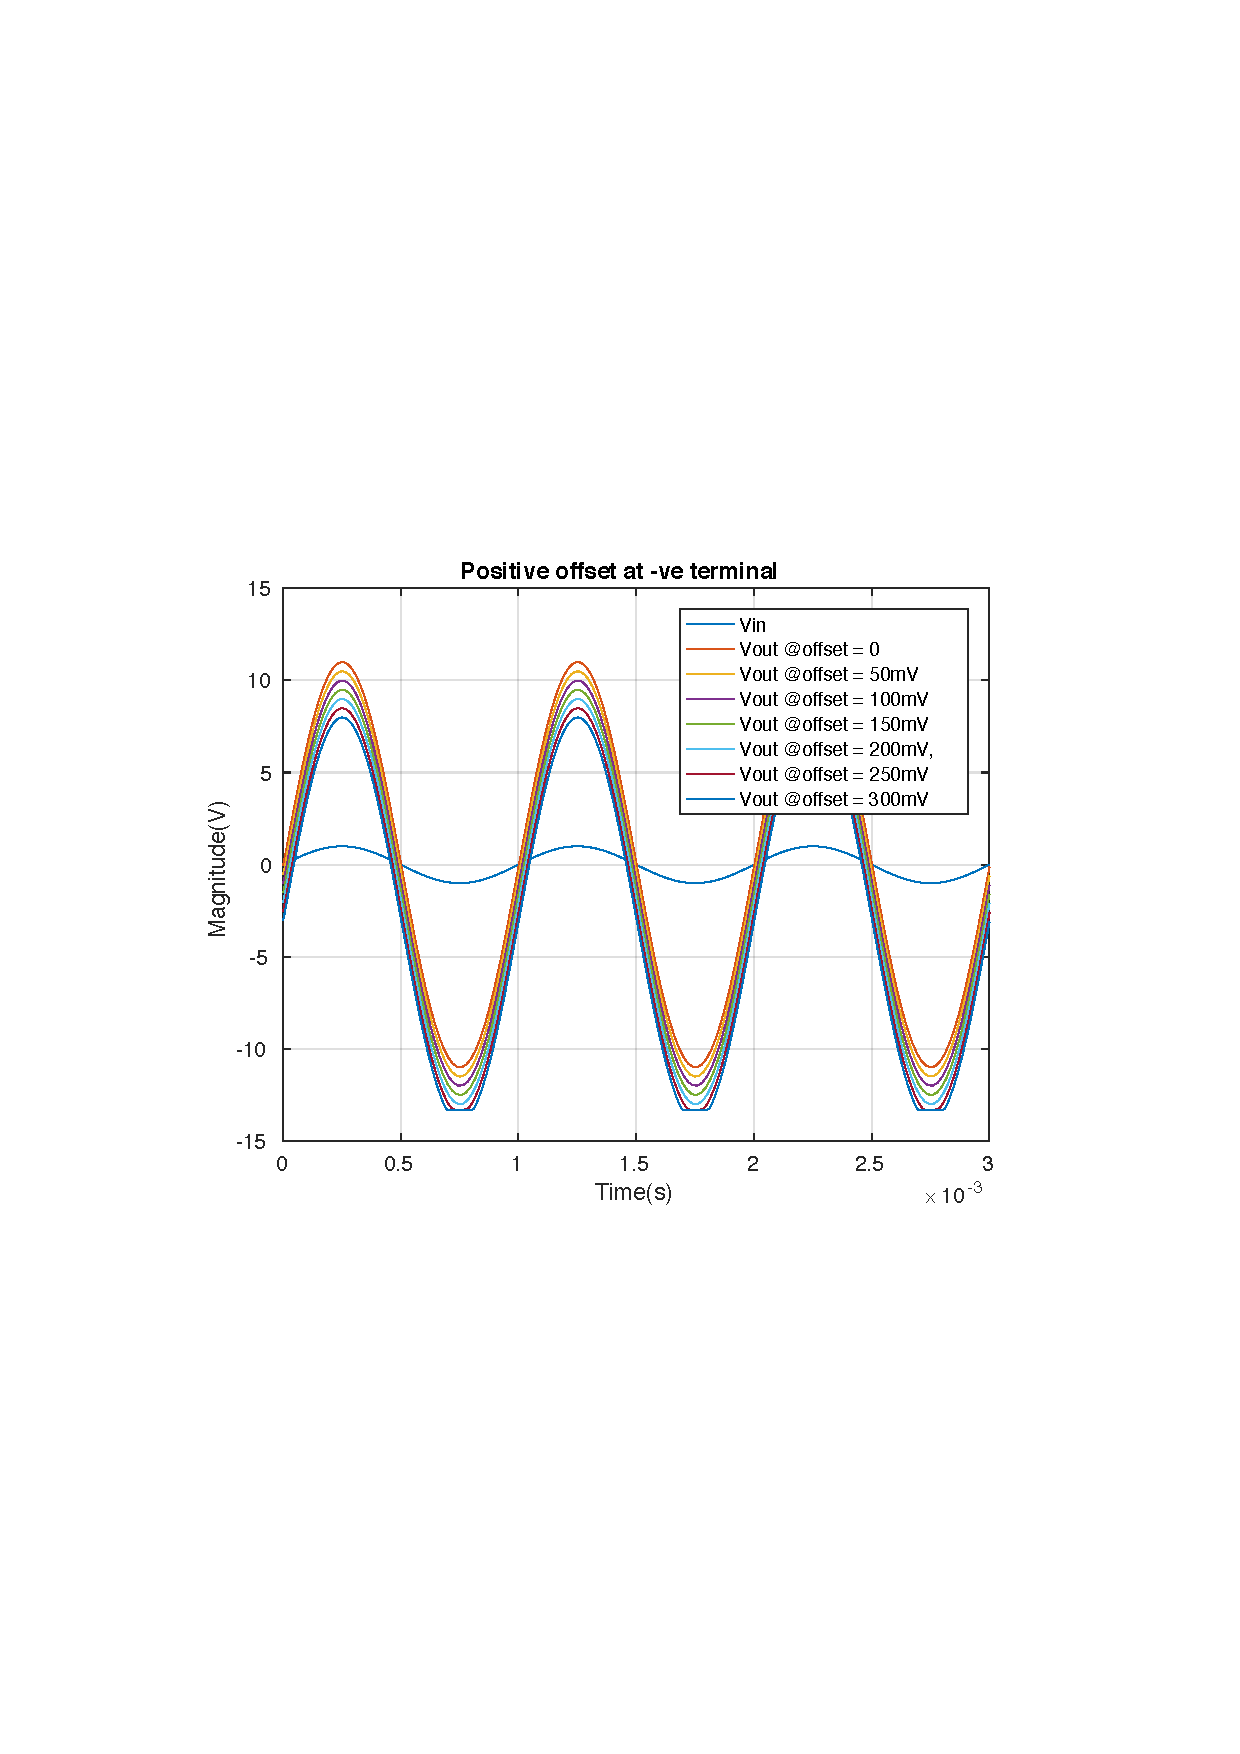
\includegraphics[width=0.9\textwidth]{img/1a_offset_pos.pdf} 
  \caption{Vout with +ve offset at -ve terminal}
  \label{pos_offset} 
\end{figure}

From figure \ref{pos_offset} and \ref{neg_offset}, it is seen that DC-offset interval is -300 mV to 200 mV. When the offset is beyong this interval the ouput saturates to either +ve or -ve supply rail. \\
%% Task 1b
\subsection{AC Analysis}

\begin{figure} [htbp]
  \centering 
  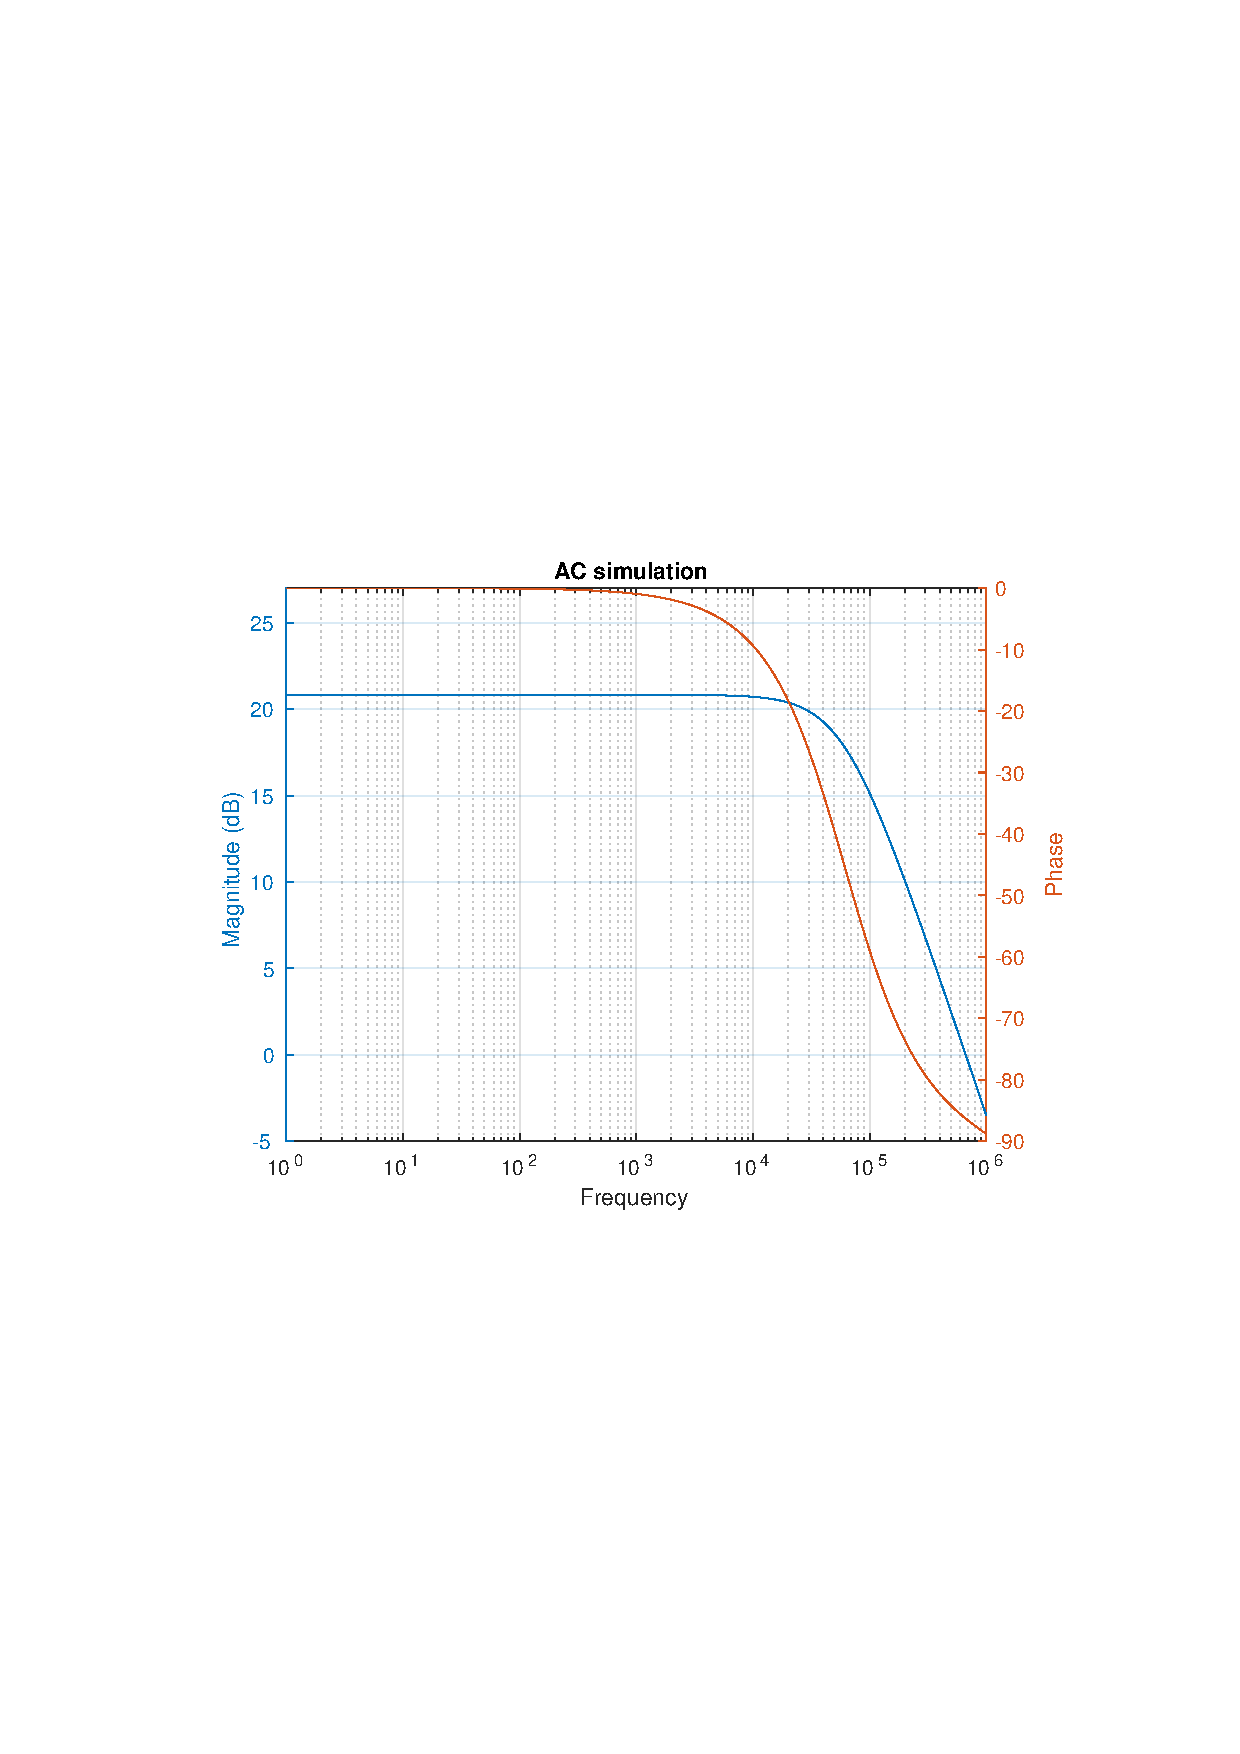
\includegraphics[width=\textwidth]{img/1b.pdf} 
  \caption{AC analysis of given opamp}
  \label{ac_ana} 
\end{figure}

%% Task 1c
\subsection{DC-offset}
\begin{figure} [htbp]
  \centering 
  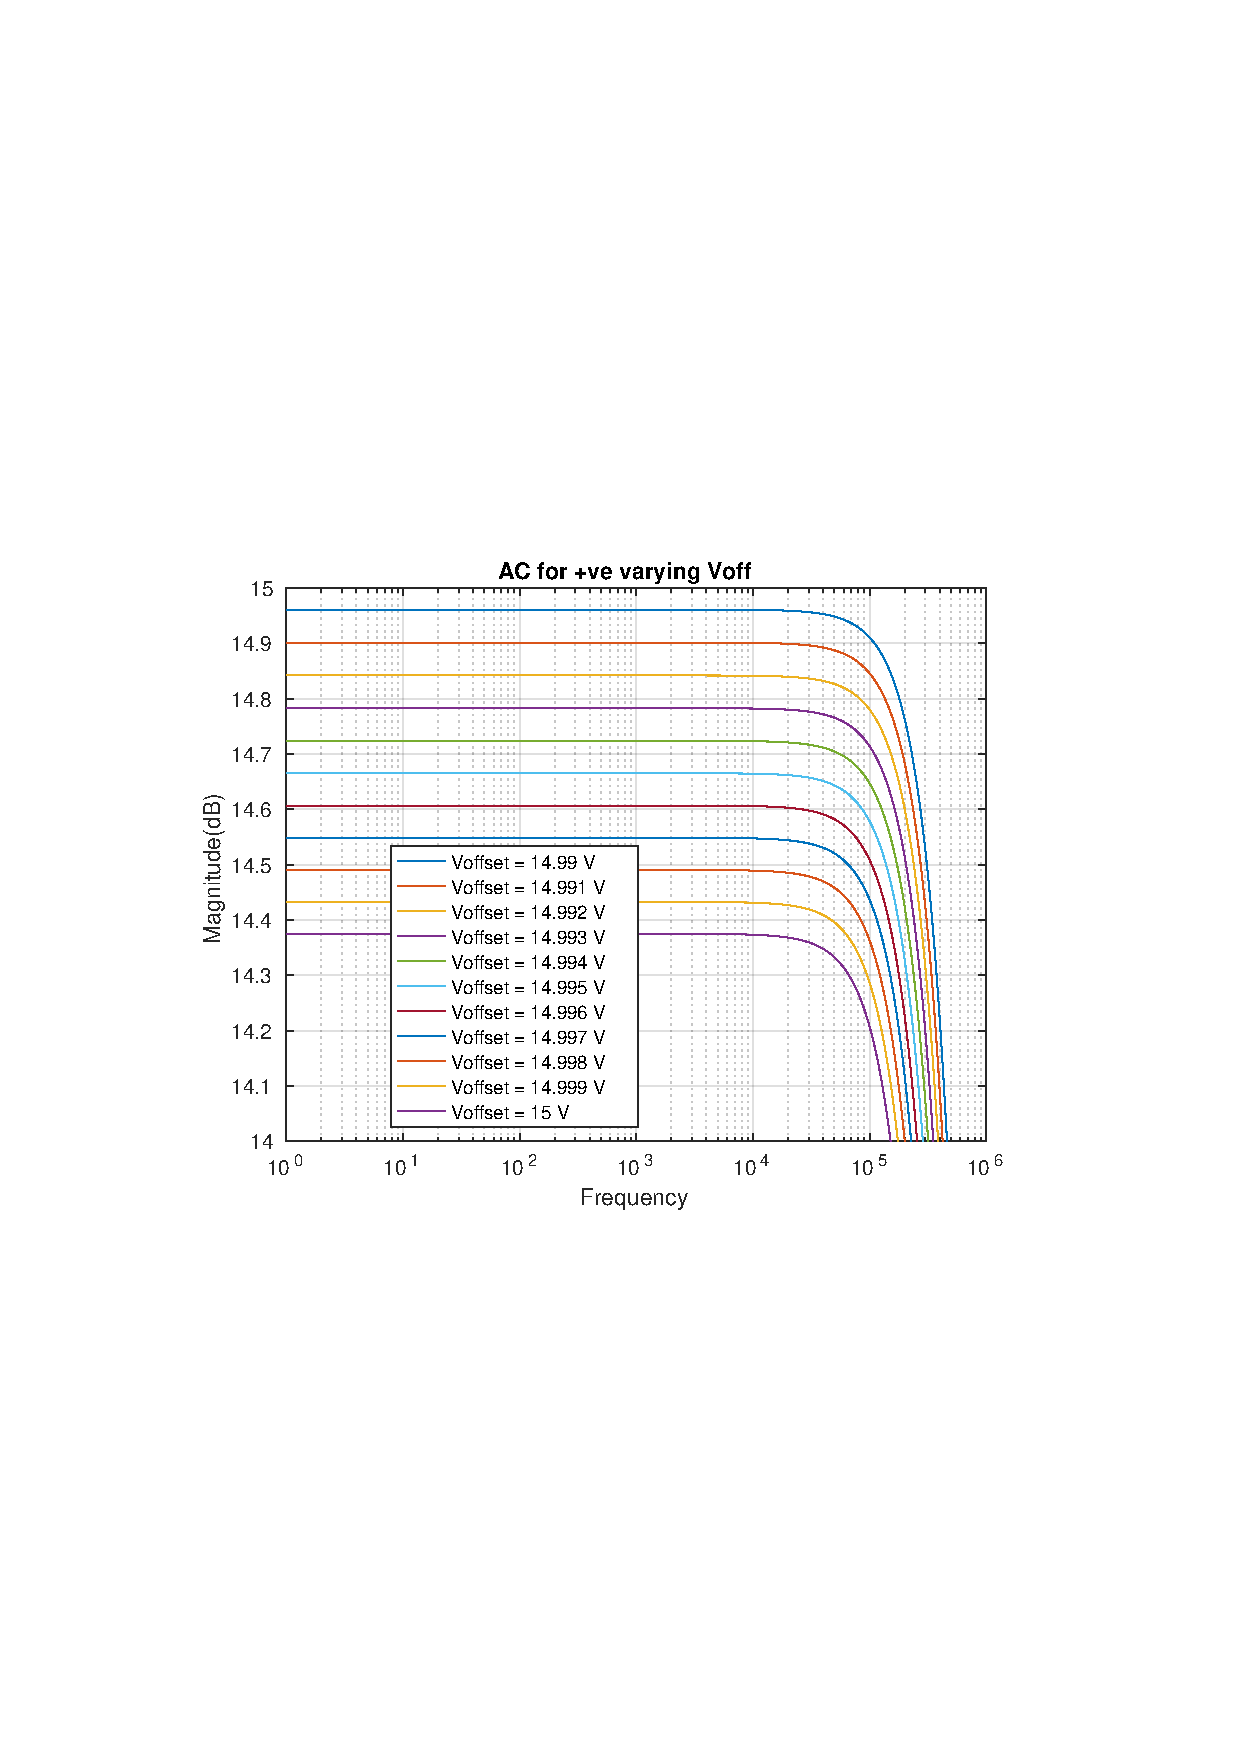
\includegraphics[width=\textwidth]{img/1c_pos_offset.pdf} 
  \caption{AC analysis with varying +ve offset}
  \label{ac_pos} 
\end{figure}

\begin{figure} [htbp]
  \centering 
  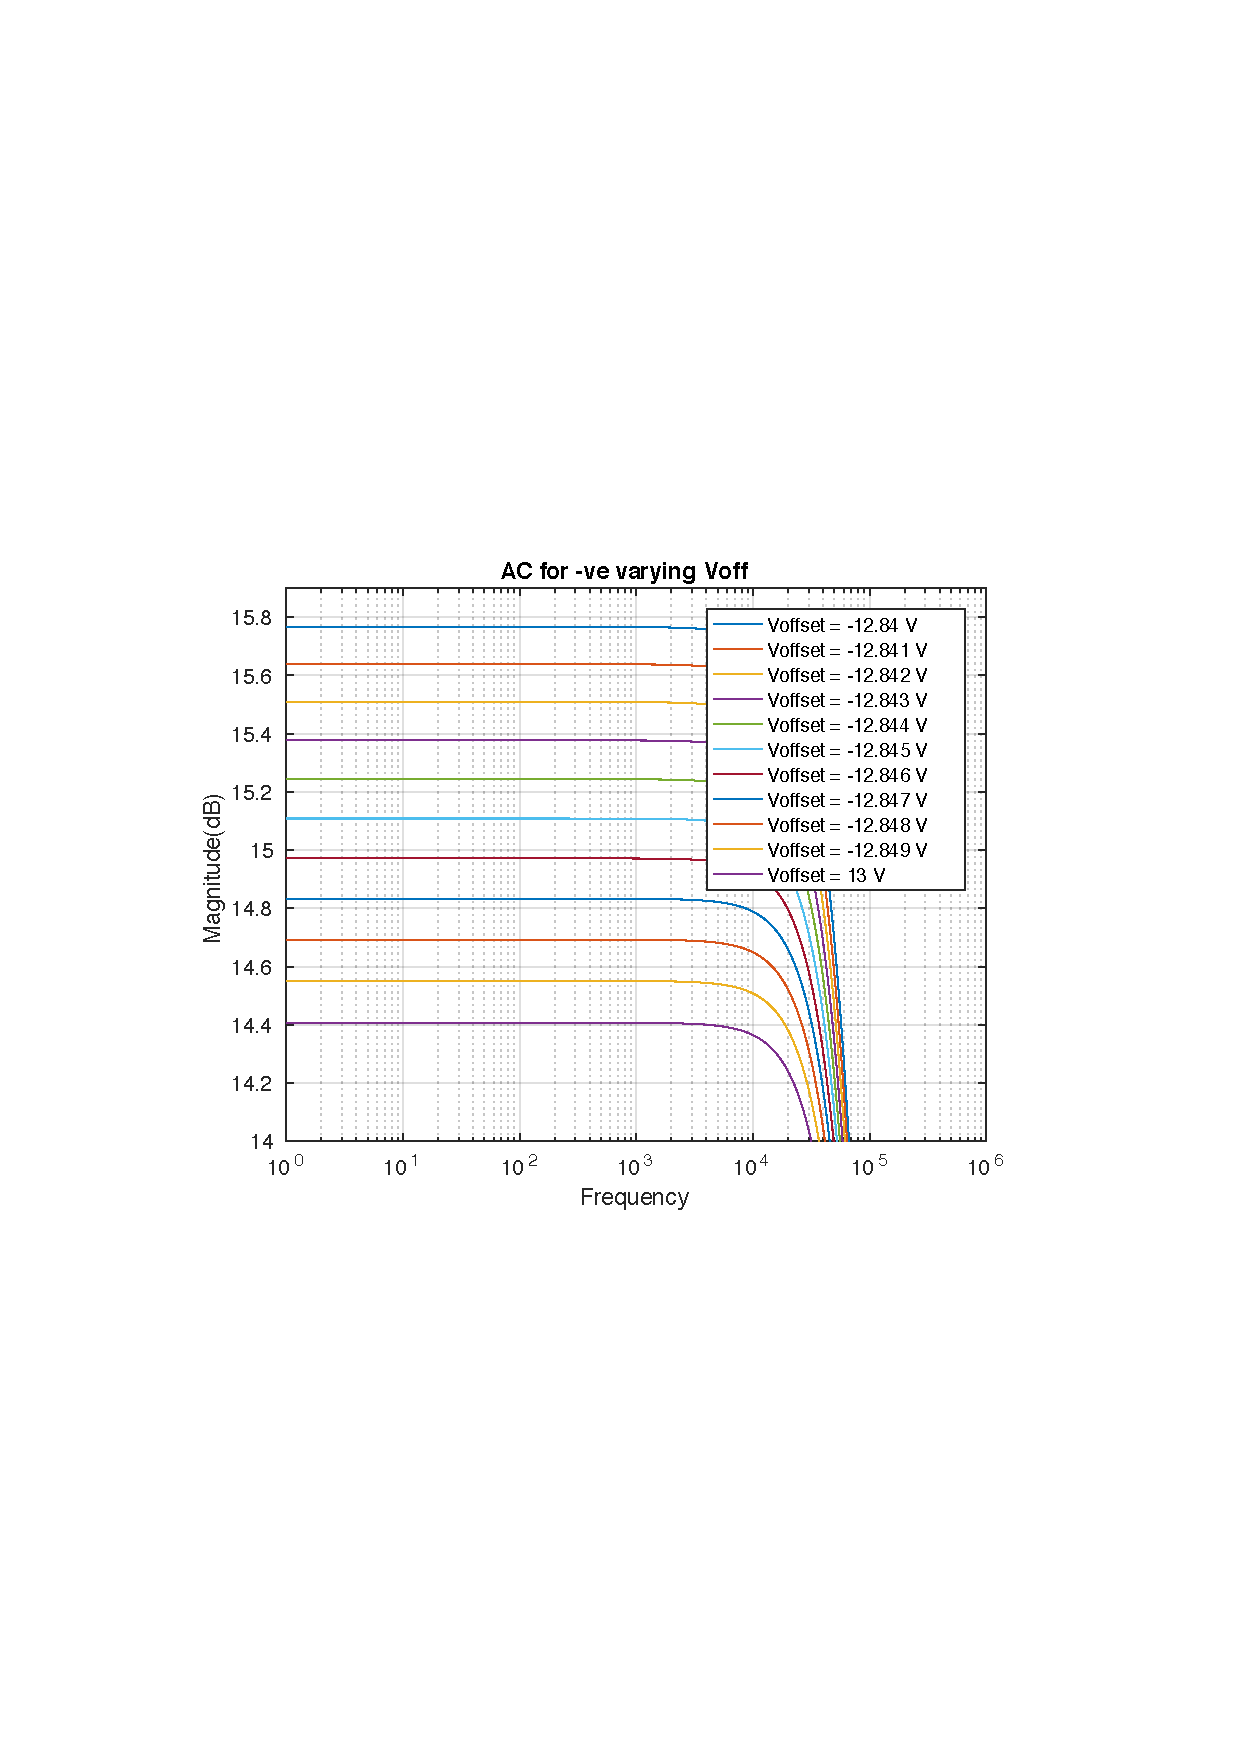
\includegraphics[width=\textwidth]{img/1c_neg_offset.pdf} 
  \caption{AC analysis with varying -ve offset}
  \label{ac_neg} 
\end{figure}

%% Task 1d
\subsection{Load capacitance }
\begin{figure} [htbp]
  \centering 
  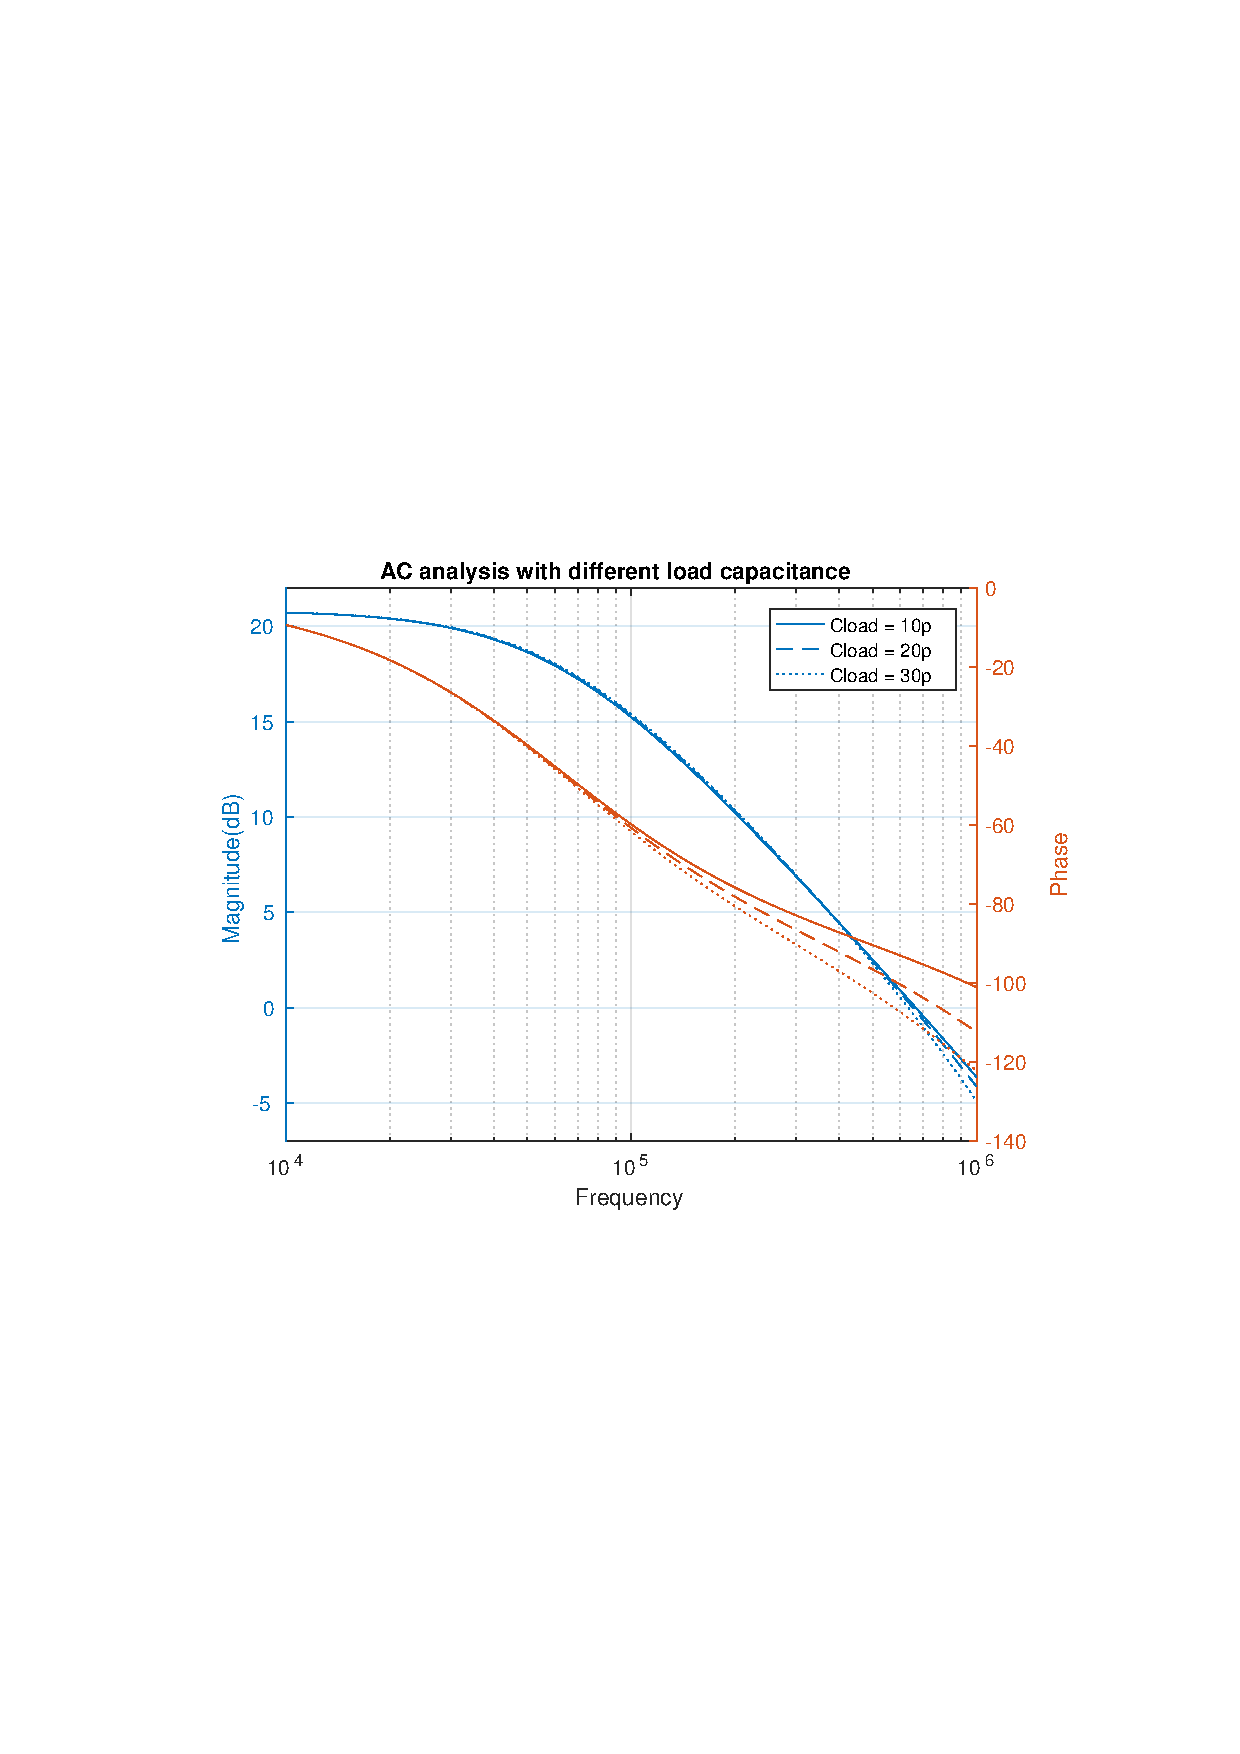
\includegraphics[width=\textwidth]{img/1d.pdf} 
  \caption{AC analysis with different load capacitance}
  \label{ac_cload} 
\end{figure}

%% Task 2
\section{Frequency charactersitcs of some curves}
%% Task 2a
\subsection{FFT}

\begin{figure} [htbp]
  \centering 
  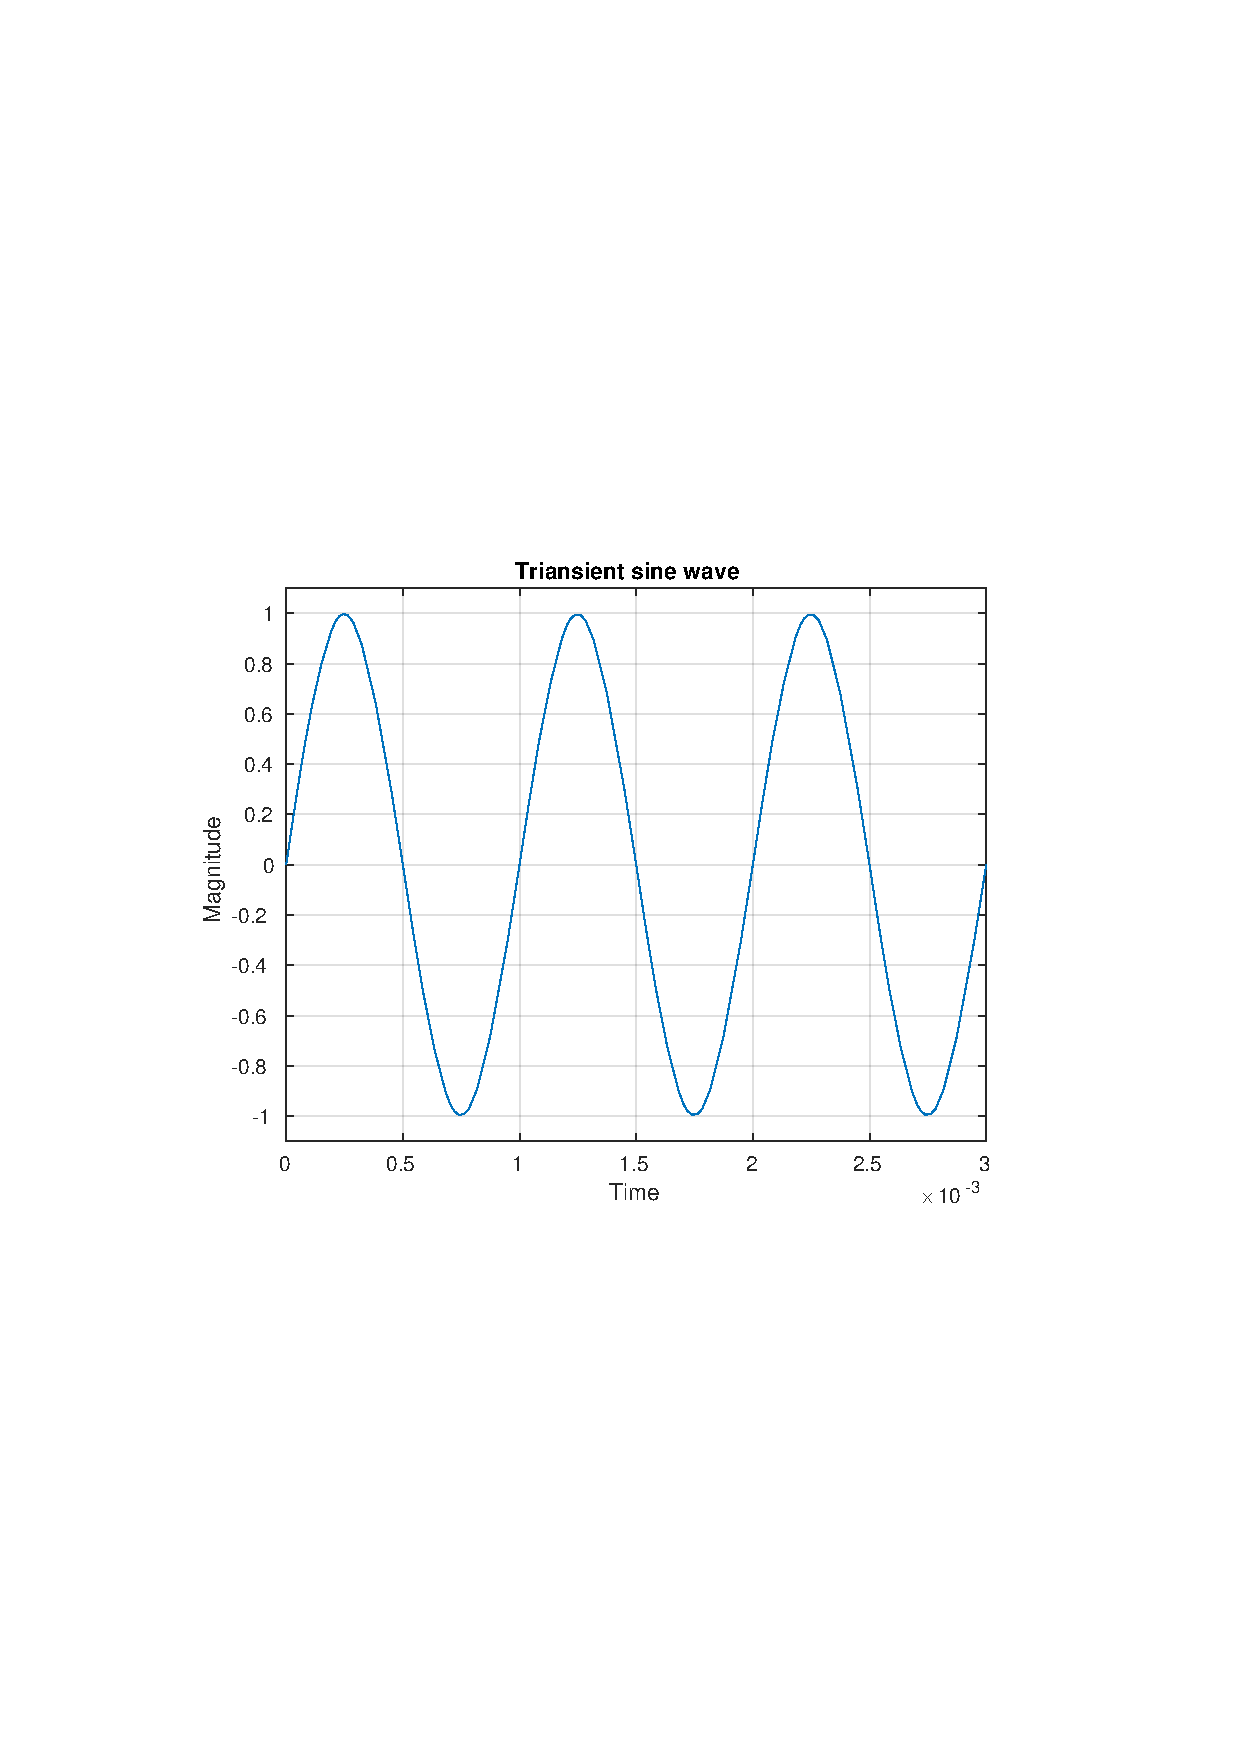
\includegraphics[width=\textwidth]{img/2a_tran.pdf} 
  \caption{Sine wave}
  \label{tran_sin} 
\end{figure}

\begin{figure} [htbp]
  \centering 
  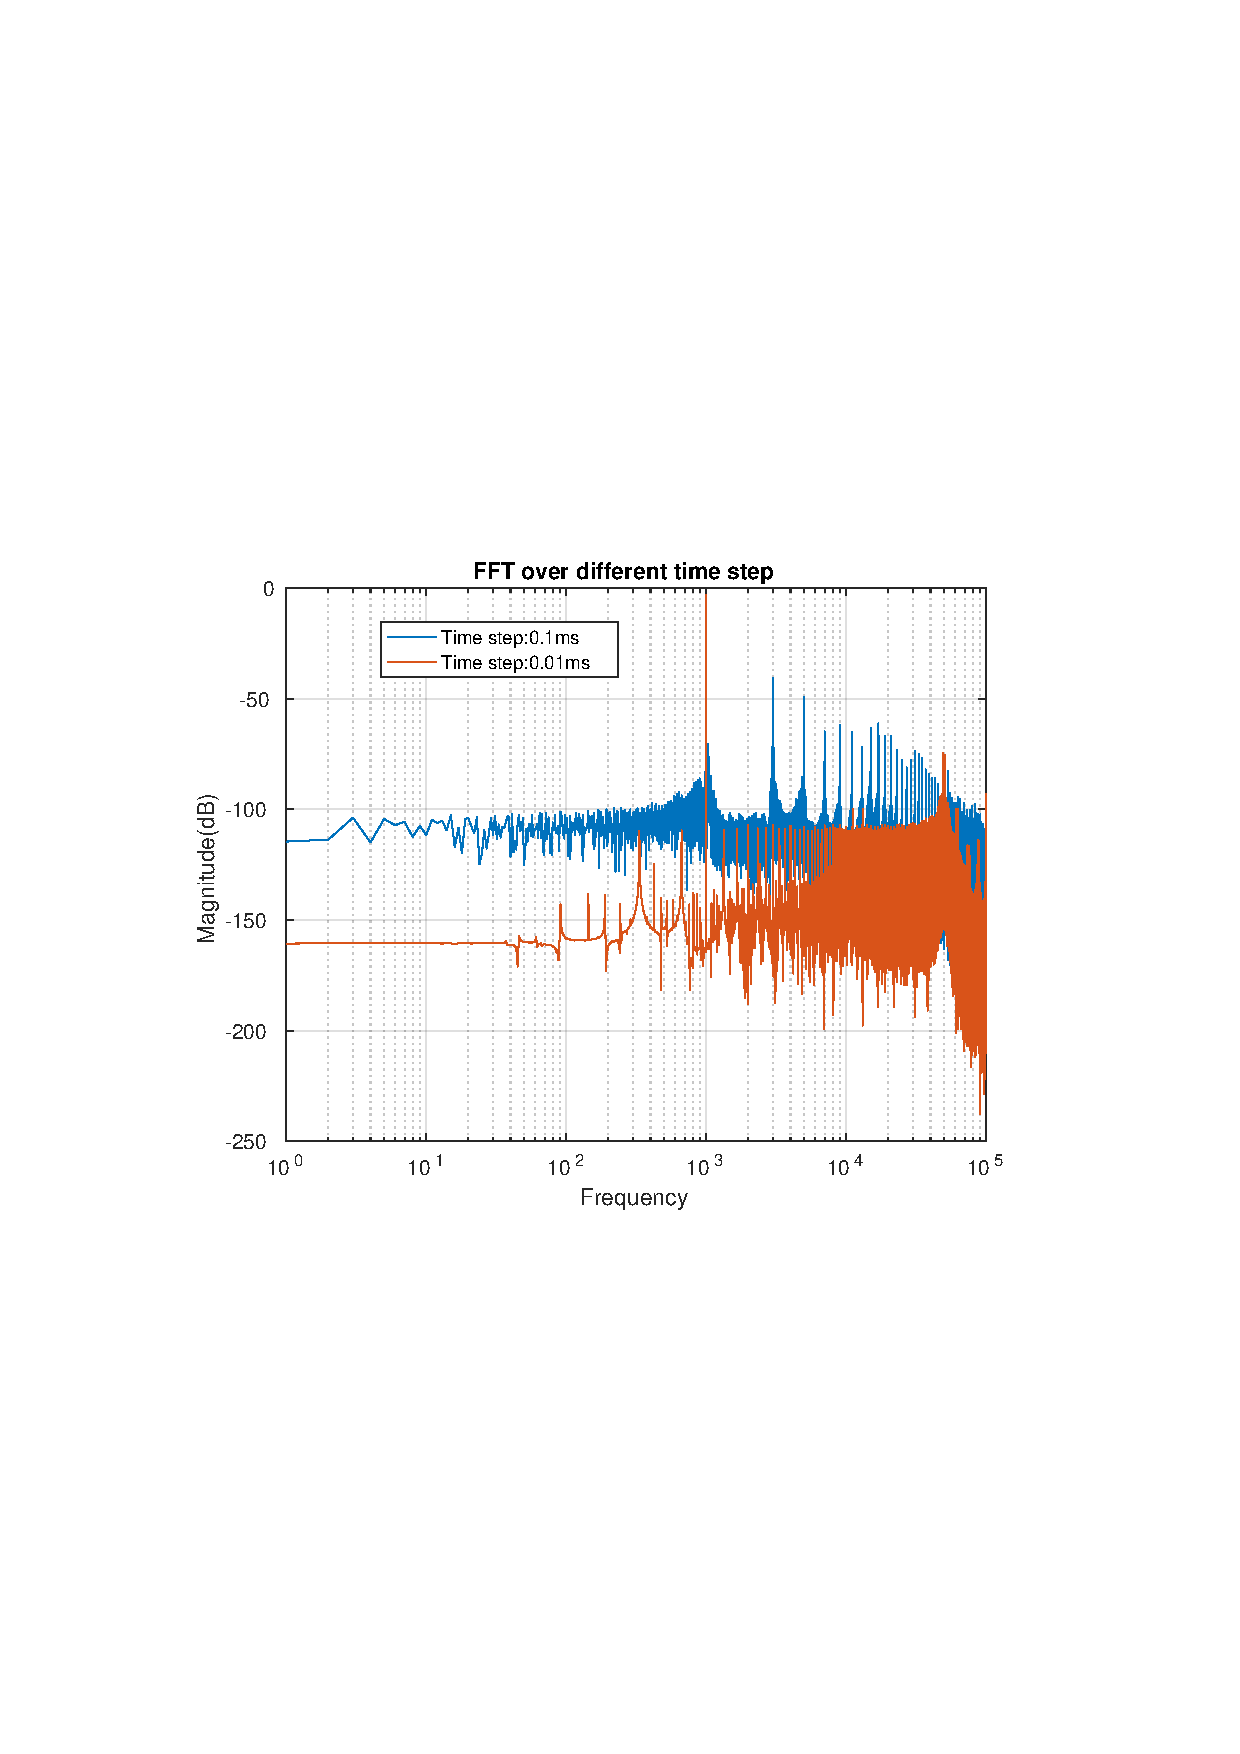
\includegraphics[width=\textwidth]{img/2a.pdf} 
  \caption{FFT of \ref{tran_sin} with different time step}
  \label{fft_sin} 
\end{figure}
%% Task 2b
\subsection{FFT-2}

\begin{figure} [htbp]
  \centering 
  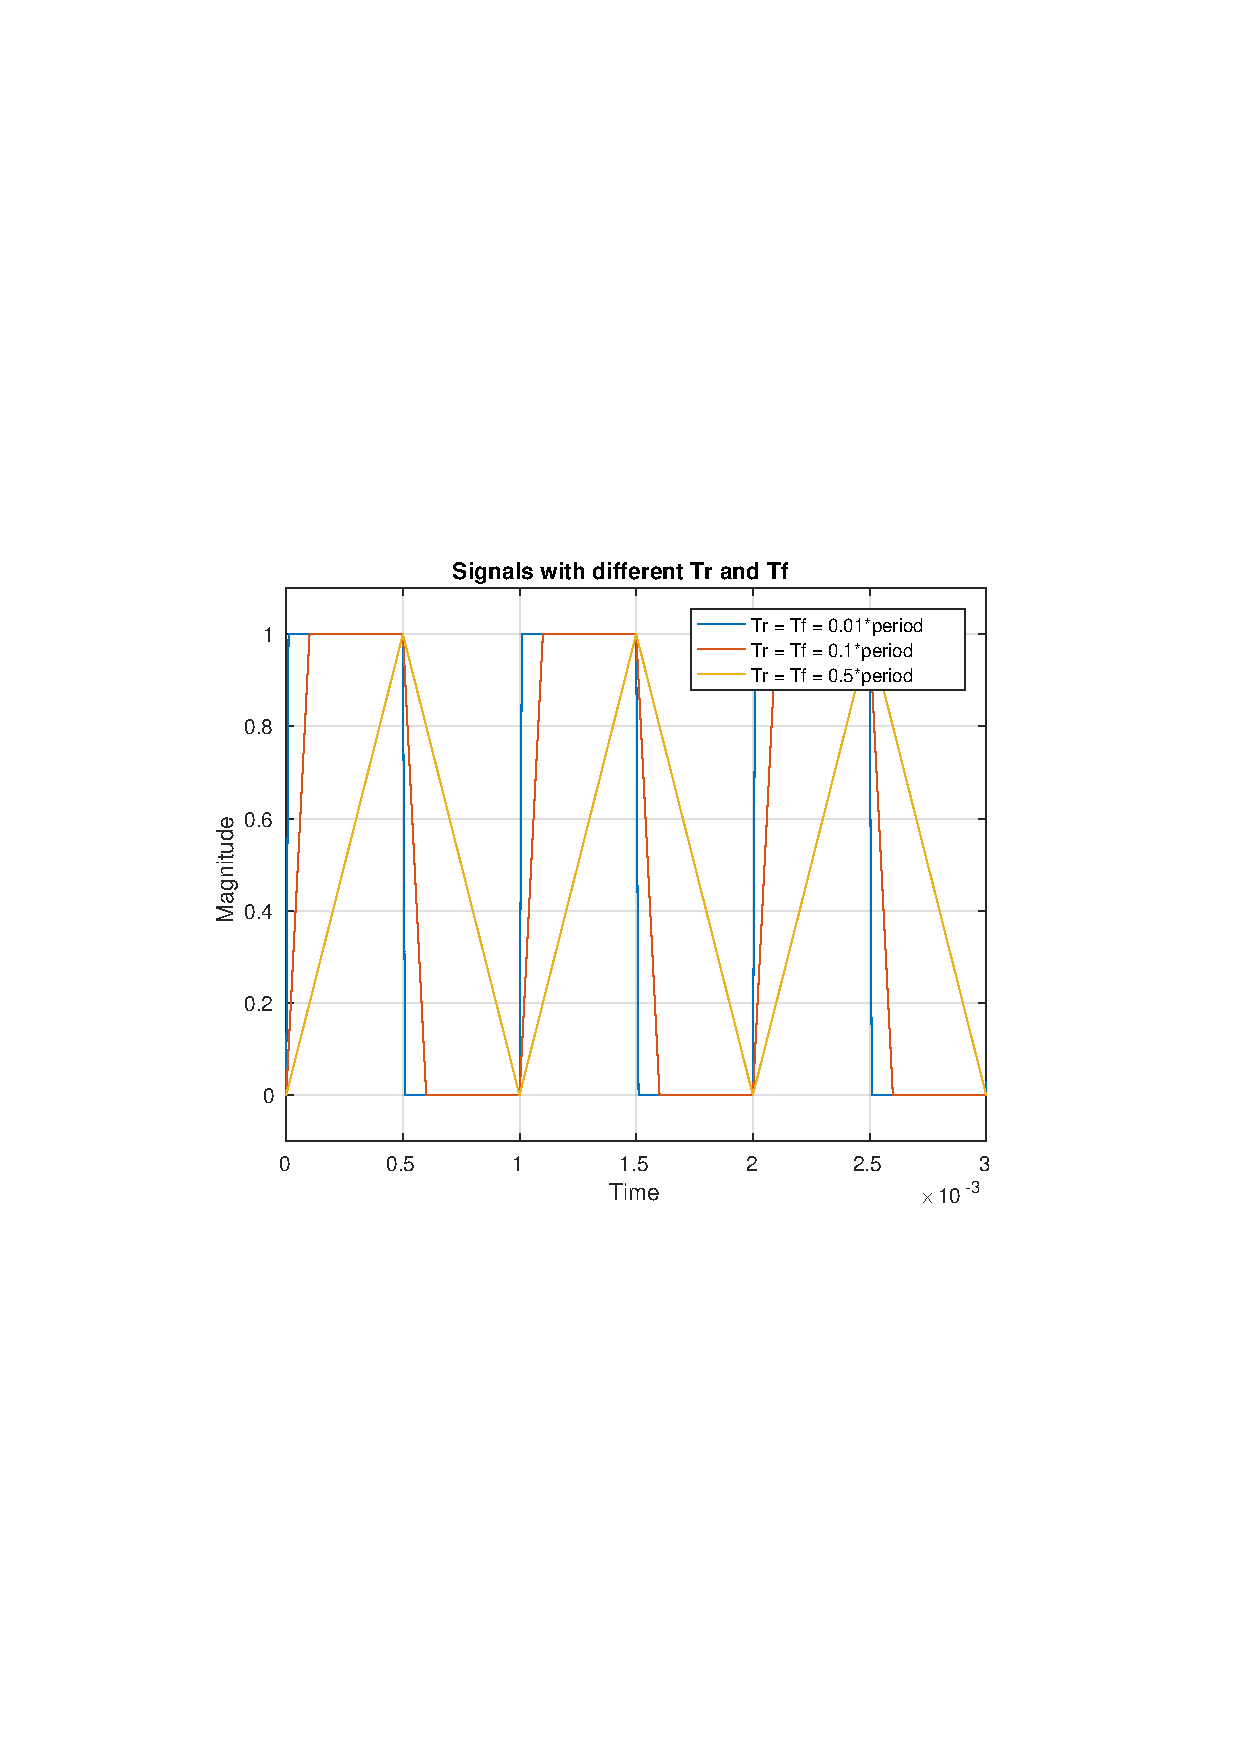
\includegraphics[width=\textwidth]{img/2b_tran.pdf} 
  \caption{Signals with different rise and fall time}
  \label{tran_all} 
\end{figure}

\begin{figure} [htbp]
  \centering 
  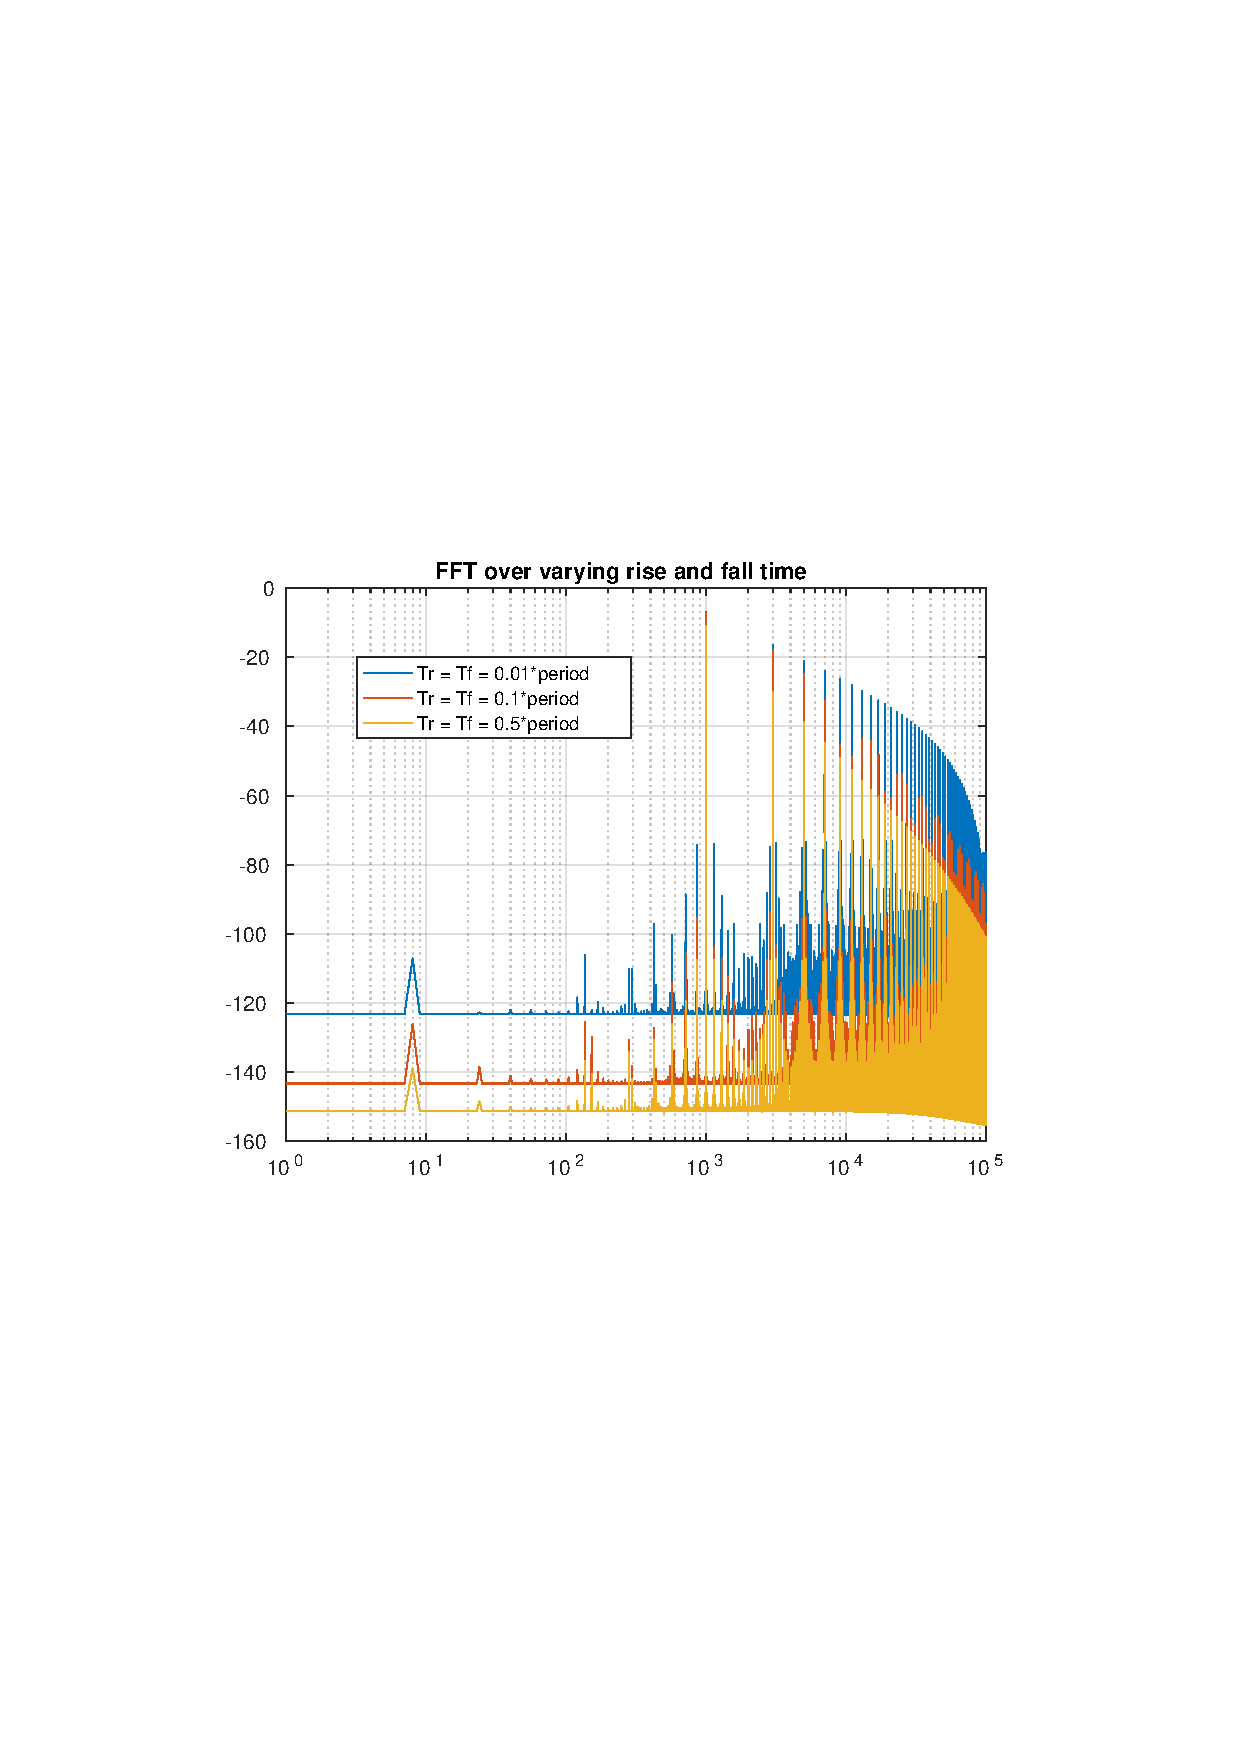
\includegraphics[width=\textwidth]{img/2b_fft.pdf} 
  \caption{FFT of \ref{tran_all} signals}
  \label{fft_all} 
\end{figure}
%% Task 2c
\subsection{Tuning}

\begin{figure} [htbp]
  \centering 
  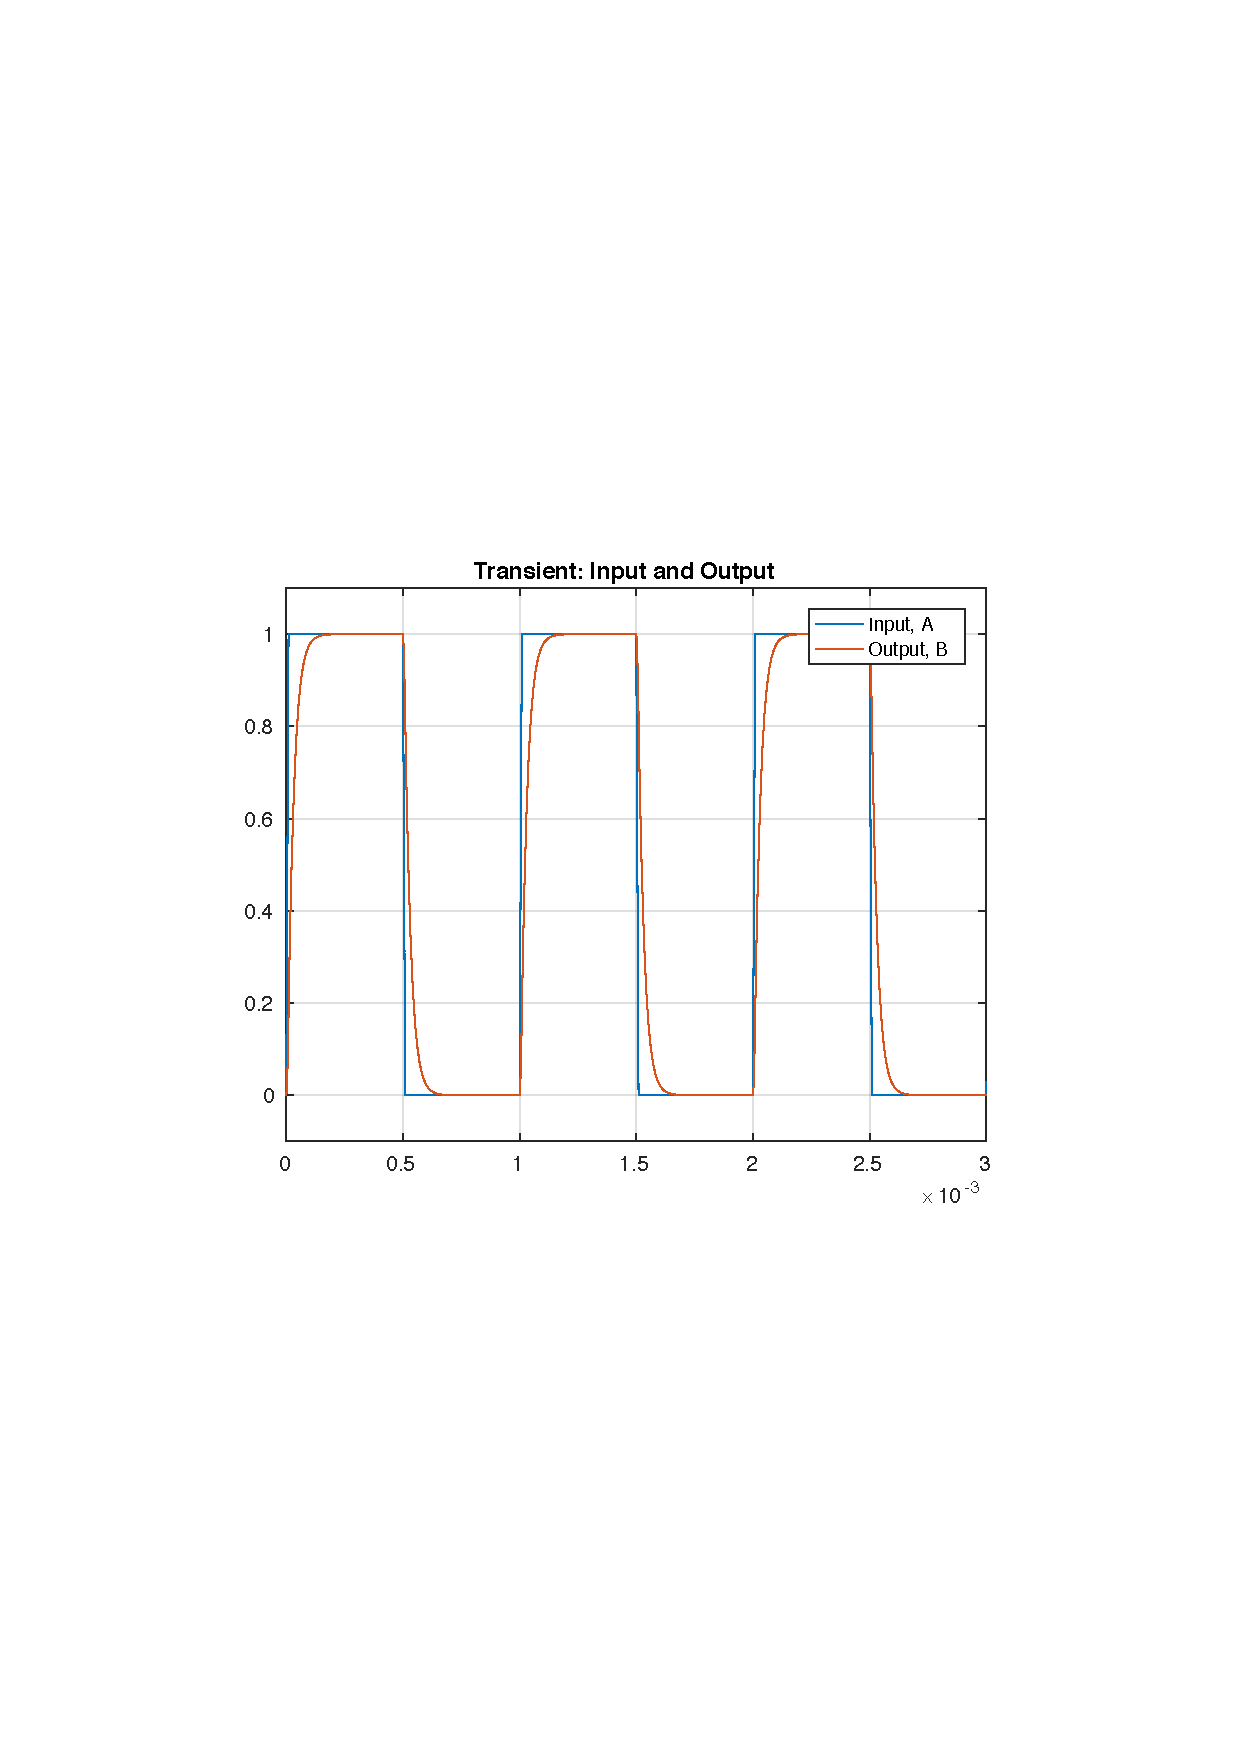
\includegraphics[width=\textwidth]{img/2c_tran.pdf} 
  \caption{Input and output of LP filter}
  \label{tran_tuned} 
\end{figure}

\begin{figure} [htbp]
  \centering 
  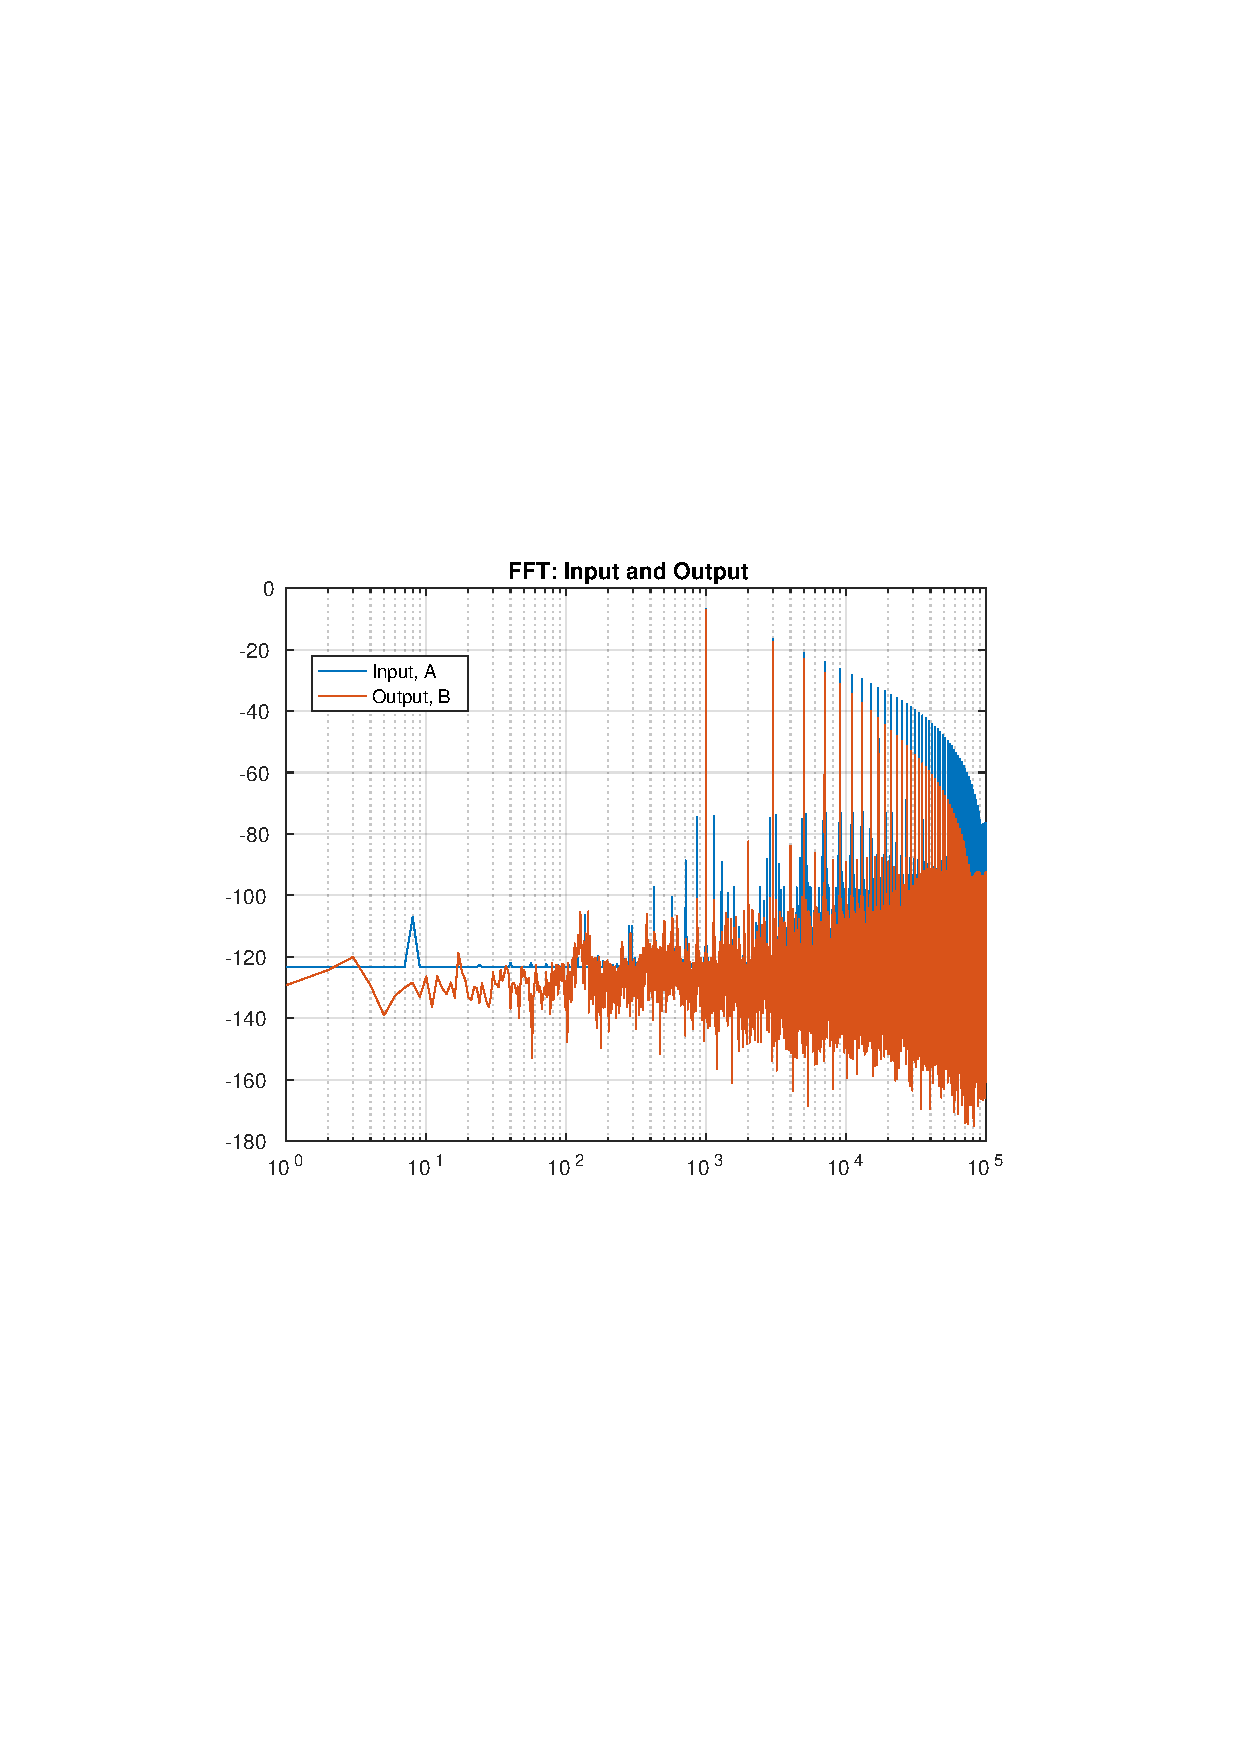
\includegraphics[width=\textwidth]{img/2c_fft.pdf} 
  \caption{FFT of \ref{tran_tuned} signals}
  \label{fft_tuned} 
\end{figure}

%% Task 3
\section{Decoupling capacitors}
Given L = 10 nH for each capacitor, traingular wave with Vpp 0-1A, Tr = Tf = 5ns, Ton = 0, period = 10us, to be stable within 5\% of 1.5V, lower corner frequency at 1MHz. 
%% Task 3a
\subsection{a}
Low frequency target impedance $Zt= k dV/dI$ where k is 2, dV is 0.075 and dI is 1A, hence 0.15 Ohm.

\subsection{b}
$n = 2L/Z_tt_r$, where L is 10nH, tr is 5 ns 27, L of each is 270nH

\subsection{c}
Also Xc must be < Zt 1.1 uF which is 40nF for each.
\subsection{d}
\subsection{f}
\subsection{f}

\section{Parasitic capacitive coupling}
\subsection{Noise captured}
\subsection{Noise after shielding}

\section{Artificial source of transient analysis}
\subsection{BV sources}
\subsection{BV sources-2}
\subsection{BV source file-1}
\subsection{Bv source file-2}

\end{document}
